
%%%%%%%%%%%%%%%%%%%%%%%%%%%%%%%%%%%%%%%%
%%%%%%%%%%%%%%%%%%%%%%%%%%%%%%%%%%%%%%%%

\chapter{Les financements non r\'ecurrents}
\label{financement-projets}

%%%%%%%%%%%%%%%%%%%%%%%%%%%%%%%%

\index{Agence nationale de la recherche (ANR)}
\index{Etablissement public \`a caract\`ere administratif \\(EPA)}
\index{Groupement d'int\'er\^et public (GIP)}

A noter que les financements non r\'ecurrents font souvent l'objet d'un
pr\'el\`evement des {\'e}tablissements dont les fonds servent \`a la gestion des contrats,
des programmes de l'ANR, {\em etc.}


\section{L'agence nationale de la recherche (ANR)}

L'ANR est un \'etablissement public \`a caract\`ere administratif (EPA),
cr\'e\'e\footnote{\`A partir d'un groupement d'int\'er\^et public (GIP) du m\^eme nom
qui existait depuis le 7 f\'evrier 2005.} le 1\ier{} janvier 2007
dans le but de financer des projets de recherche ({\em cf.}, \href{https://www.legifrance.gouv.fr/loda/id/LEGITEXT000006054155}{D\'ecret n°2006-963 du 1 ao\^ut 2006 portant organisation et fonctionnement de l'Agence nationale de la recherche}).

Le financement sur projets \'etant un m\'ecanisme
r\'epandu \`a l'\'echelle internationale,
l'objectif de l'ANR est d'accro\^\i  tre le nombre de projets de
recherche venant de toute la communaut\'e scientifique, financ\'es
apr\`es mise en concurrence et \'evaluation par les pairs.
L'ANR s'adresse \`a la fois aux \'etablissements publics de recherche
et aux entreprises, avec une double mission~: produire de nouvelles
connaissances et favoriser les interactions entre laboratoires
publics et laboratoires d'entreprise en d\'eveloppant les
partenariats.

\textbf{Lien utile\hspace{.5em}} \url{https://anr.fr//}

\subsection{Fonctionnement g\'en\'eral}

L'ANR finance les projets au travers d'appels d'offre (AAP). Ces projets, apr\`es s\'election, sont accord\'es pour une dur\'ee de 3 {\`a} 4 ans. Les appels d'offre ont \'evolu\'e depuis la cr\'eation de l'ANR. Pour l'essentiel (les appels d'offre g\'en\'eriques), les projets financ\'es correspondent \`a des programmes th\'ematiques organis\'es autours de 9 {\em d\'efis soci\'etaux} ou au programme {\em d\'efi des autres savoirs}. Les projets se r\'epartissent en deux cat\'egories~:
\begin{itemize}
\item la cat\'egorie `chercheurs et chercheuses', qui concerne les projets pour {\em jeunes chercheuses et jeunes chercheurs} financ\'es par l'instrument du m\^eme nom (JCJC). Ce sont des projets destin\'es \`a financer les recherches d'un\mp e jeune CR ou MCF qui cherche {\`a} prendre son autonomie scientifique avec constitution d'une petite {\'e}quipe autour de elle/lui.
\item la cat\'egorie `recherche collaborative', qui concerne les projets de grande ampleur, en collaboration avec plusieurs \'equipes de recherche publiques ou priv\'ees, nationales ou internationales. Parmi les instruments de financement de ces projets on trouve les {\em projets de recherche collaborative} (PRC), les {\em projets de recherche collaborative internationale} (PRCI) et les {\em projets de recherche collaborative - entreprise} (PRCE).
\end{itemize}

Les r\`egles de financement, ainsi que les crit\`eres
d'\'evaluation, peuvent varier d'un instrument \`a l'autre. %Nous reviendrons plus loin sur le cas des projets JCJC.

Ces programmes sont ouverts \`a toutes les disciplines et donc, entre autres,
aux math\'ematiques. Un certain nombre de programmes th\'ematiques
peuvent l\'egitimement justifier la participation de math\'ematicien(ne)s (notamment le d\'efi 7, {\em Soci\'et\'e de l'information et de la communication}).
Il ne faut donc pas h\'esiter \`a r\'epondre
\`a un appel \` a projets au sein d'une \'equipe pluridisciplinaire. De plus, il est tout \`a
fait possible de candidater sur plusieurs programmes en m\^eme temps.

Les projets s\'electionn\'es peuvent permettre de financer des d\'epenses d'\'equipement\footnote{On entend par \'equipement du mat\'eriel dont le co\^ut est sup\'erieur \`a 4000\,\euro~(machines de calcul par exemple).}, des d\'epenses de fonctionnement\footnote{Ce sont toutes les d\'epenses qui ne sont ni les salaires, ni l'\'equipement : missions, ordinateurs personnels, organisation de workshops, {\em etc.}}, des recrutements de personnel sous contrat \`a dur\'ee d\'etermin\'ee (doctorant\mp e\mp s, post-doctorant\mp e\mp s, ing\'enieur\mp e\mp s
d'\'etude), des d\'echarges d'enseignement pour les EC (uniquement pour le financement JCJC), ainsi que des prestations de services externes.

\subsection{Calendrier}

L'ANR publie chaque ann\'ee, \`a la fin de l'\'et\'e, un document d\'etaillant son {\em plan d'action} pour l'ann\'ee \`a venir. C'est ce document qui d\'efinit les grands th\`emes qui seront financ\'es.

Le calendrier et les modalit\'es de d\'ep\^ot des projets sont quant \`a eux fix\'es dans un second document, {\em l'appel \`a projets g\'en\'erique}. Depuis 2014, la soumission et l'\'evaluation d'un projet s'effectue en deux \'etapes :
\begin{itemize}
\item la pr\'eproposition (hors PCRI) : elle recueille les informations pratiques du projet (nom, montant de l'aide demand\'ee, \'equipe, CV du\mp de la porteur\mp se) ainsi qu'un descriptif scientifique du projet (d'environ 2-3 pages). La pr\'eproposition est g\'en\'eralement soumise en {\bf octobre} et les r\'esultats de l'\'evaluation sont connus en f\'evrier-mars. La d\'ecision de s\'election pour passer en phase 2 est prise, au mois de Janvier. Ces trois derni\`eres ann\'ees, le taux de s\'election en nombre de projets a \'et\'e de l'ordre de 40\%. Les porteur\mp ses des projets s\'electionn\'es soumettent alors une proposition d\'etaill\'ee. 
\item la proposition d\'etaill\'ee : elle contient le coeur du projet scientifique. C'est un document de 20 pages d\'etaillant le contexte du projet, les objectifs \`a atteindre et les moyens mis en oeuvre, l'organisation de l'\'equipe, ainsi que l'impact et les retomb\'ees du projet. Cette proposition est soumise en {\bf avril} et les r\'esultats de l'\'evaluation sont publi\'es dans l'\'et\'e.
\end{itemize}

Ces dates sont indicatives et susceptibles de varier d'une ann\'ee \`a l'autre. Nous vous conseillons de vous rendre sur le site de l'ANR pour obtenir les informations \`a jour.

\subsection{Pour les jeunes -- L'instrument {\em Jeunes Chercheuses et Jeunes Chercheurs} (JCJC)}

Les jeunes chercheur\mp euse\mp s qui souhaitent \^etre porteur\mp se d'un projet sont surtout concern\'e\mp e\mp s par le programme JCJC.
%Pour suivre l'actualit\'e des appels \`a projets, nous vous conseillons de consulter r\'eguli\`erement le site de l'ANR ({\em cf.} plus haut).

\index{Agence Nationale de la Recherche (ANR)!Programme {\em Jeunes Chercheuses et Jeunes Chercheurs}}

\subsection*{Les objectifs}

L'objectif de l'instrument de financement {\em Jeunes Chercheuses et Jeunes Chercheurs} (JCJC) est de pr\'eparer la nouvelle g\'en\'eration de jeunes chercheur\mp euse\mp s de talents appel\'e\mp e\mp s \`a devenir les futurs leaders ou dirigeant\mp e\mp s de la recherche scientifique fran\c{c}aise. Il s'agit donc de favoriser la prise de responsabili\'e par des jeunes chercheur\mp euse\mp s et de les inciter \`a s'attaquer \`a des verrous scientifiques ou technologiques avec des approches originales.

L'instrument vise \`a permettre \`a la jeune chercheur\mp euse de d\'evelopper sa propre th\'ematique de recherche, de consolider son \'equipe ou d'en constituer une, d'acqu\'erir une culture de la recherche sur projet et d'exprimer rapidement ses capacit\'es d'innovation. Il s'agit \'egalement d'un tremplin pour les jeunes chercheur\mp euse\mp s fran\c{c}ais\mp e\mp s qui, gr\^ace \`a une premi\`ere aide de l'ANR, pourront plus facilement envisager de d\'eposer un projet en r\'eponse aux appels du Conseil europ\'een  de la recherche (ERC), et ceci avec de meilleures chances de succ\`es. Cibl\'e sur l'individu, cet instrument pr\'evoit le financement de la seule \'equipe du jeune chercheur ou de la jeune chercheuse.

Il faut n\'eanmoins garder \`a l'esprit que les appels \`a projets ERC \emph{starting grants} sont r\'eserv\'es aux jeunes chercheur\mp euse\mp s ayant soutenus leur th\`ese au maximum 7 ans avant la date de soumission du projet, contre 10 ans pour les JCJC.

%En 2016, les financements accord\'es sur une p\'eriode de quatre ans \'etaient en moyenne de 130\,k\euro{} (contre 80\,k\euro{} en 2011, voir la figure \ref{fig:anr}).

\subsection*{Les crit\`eres d'\'evaluation}

Les projets (pr\'epropositions et propositions d\'etaill\'ees) sont \'evalu\'ees \`a la fois par des expert\mp e\mp s du domaine concern\'e par le projet, et d'un comit\'e d'\'evaluation scientifique (CES). Depuis 2014, c'est le CES 40 (math\'ematiques et informatique) qui est en charge des projets math\'ematiques issus du d\'efi des autres savoirs et du d\'efi 7 (Soci\'et\'e de l'information et de la communication).

Les crit\`eres d'\'evaluation varient selon les appels \`a projet, et nous vous conseillons de vous r\'ef\'erer aux informations mises \`a jour sur le site de l'ANR. Pour les projets JCJC, outre la qualit\'e du projet, il sera toujours tr\`es important de mettre l'accent sur la {\bf prise d'autonomie} des jeunes chercheur\mp euse\mp s. Ainsi, il faut \'eviter de faire participer un\mp e ou des chercheur\mp euse\mp s seniors \`a ces projets, et tout particuli\`erement les directrices ou directeurs de th\`eses de membres du projet.

Lors de la r\'edaction du projet, notamment du document scientifique de la proposition d\'etaill\'ee, il faut veiller \`a respecter la forme souhait\'ee par l'ANR. Les projets sont \'evalu\'es selon des crit\`eres tr\`es bien d\'efinis, qu'il faut bien mettre en valeur dans le document. Nous vous conseillons de vous renseignez aupr\`es de vos coll\`egues qui ont eu r\'ecemment un projet financ\'e.

\subsection*{Sur les taux de succ\`es}

Des changements importants sont apparus en 2014 \`a l'ANR. L'agence a toujours souhait\'e faire appara\^itre les appels \`a projets g\'en\'eriques comme comp\'etitifs et donc limiter le nombre de projets s\'electionn\'es. Ainsi, l'ANR imposait un taux de s\'election vis\'e (pour les pr\'epropositions et les propositions d\'etaill\'ees).

Les disciplines th\'eoriques ont toujours eu des difficult\'es avec ce principe. Les comit\'es d'\'evaluation scientifique en math\'ematiques ont donc r\'eguli\`erement demand\'e et obtenu un assouplissement de cette r\`egle. Avant 2014, il n'\'etait pas rare d'avoir un taux de s\'election sup\'erieur \`a 30\% des demandes initiales. Il \'etait possible d'arriver \`a un tel taux gr\^ace \`a la latitude qui \'etait laiss\'ee au comit\'e pour ajuster les budgets avec une enveloppe budg\'etaire globale au comit\'e. En 2014, les r\`egles ont chang\'e :

\begin{itemize}
\item caract\`ere impos\'e du taux de s\'election (entre 10 et 12\%) sans possibilit\'e de s\'electionner plus largement avec le dispositif d\'ecrit ci-dessus ;
\item comit\'e \'elargi \`a l'informatique th\'eorique (avec certaines fois robotique, ou d'autres disciplines) ;
\item disparition des AAP non th\'ematiques au profit des AAP th\'ematiques au sein de d\'efis scientifiques. Les math\'ematiques sont depuis 2014 dans le d\'efi 7 et dans le {\em d\'efi des autres savoirs}.
\end{itemize}

Le CES 40 a donc constat\'e une nette d\'egradation du nombre de projets financ\'es en math\'ematiques \`a la suite de ce nouveau dispositif. La d\'egradation a \'et\'e extr\^emement forte en JCJC. Ceci a donc d\'ecourag\'e les jeunes MCF et CR de d\'eposer de nouveaux projets. Comme l'ANR imposait un taux de s\'election sur le nombre de projets soumis, la diminution du nombre de projets finalement s\'electionn\'es s'est acc\'el\'er\'ee. En 2016, le CES 40 a refus\'e de transmettre ses conclusions et a engag\'e un bras de fer avec l'ANR. Au terme de longues discussions, le comit\'e a obtenu gain de cause avec la libert\'e de s\'electionner des projets en plus grand nombre en ajustant les budgets des projets dans une enveloppe budg\'etaire donn\'ee. Ceci a permis au comit\'e de financer plus de projets et en particulier en JCJC : 9 projets ont \'et\'e financ\'es en 2016, contre 4 en 2014 et 2015 ({\em cf.} Figure \ref{fig:anr}).

\subsection*{Quelques chiffres}

\begin{figure}[ht!]
\resizebox{\textwidth}{!}{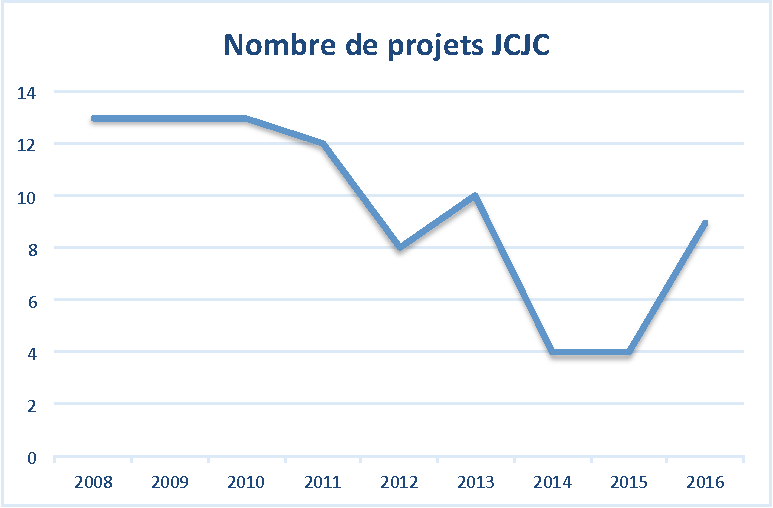
\includegraphics{Images/PastedGraphic-2.pdf}
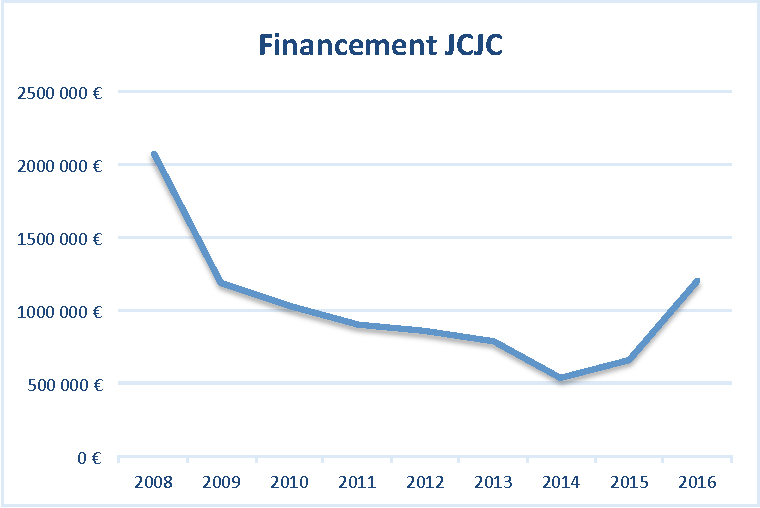
\includegraphics{Images/PastedGraphic-1.pdf}
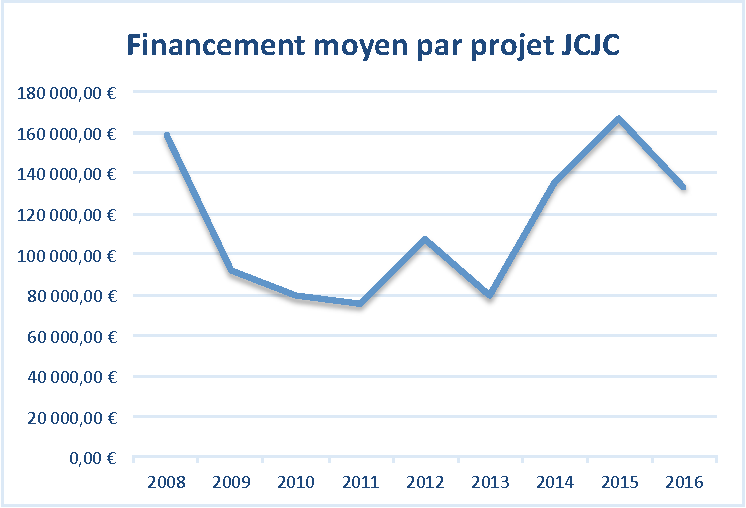
\includegraphics{Images/PastedGraphic-3.pdf}}
\caption{\'Evolution du financement JCJC}
\label{fig:anr}
\end{figure}

Concluons en remarquant que sur les deux ann\'ees 2017 et 2018 le taux de succ\`es global en nombre de projets a \'et\'e de 21,6\% pour le CES 40 mais de 17,6 \% en montant d'aide.

%%%%%%%%%%%%%%%%%%%%%%%%%%%%%%%%%%%%%%%%%%%%%%%%
%%%%%%%%%%%%%%%%%%%%%%%%%%%%%%%%%%%%%%%%%%%%%%%%

\section{Les EX: \og initiatives d'excellence\fg{} \& co.}\label{trucenex}

\subsection{Programme Investissements d'Avenir}

Le premier Programme Investissements d'Avenir (PIA1) proposait, en juillet-septembre 2010, 35 milliards d'euros, 
dont 22 milliards d'euros destin\'es \`a l'enseignement sup\'erieur et \`a la recherche.
L'ANR a {\'e}t{\'e} op{\'e}rateur du PIA1 pour tout ce qui concerne la recherche et l'enseignement sup{\'e}rieur. 
A ce titre, elle a {\'e}t{\'e} charg{\'e}e du suivi administratif et financier des projets, 
il existe d'autres op{\'e}rateurs (CEA, Caisse des D{\'e}pôts par exemple). 
%Le financement est totalement distinct du celui des projets du paragraphe pr{\'e}c{\'e}dent.
%
%Les investissements d'avenir se d\'eclinent en plusieurs \og actions\fg{}, qui sont des appels d'offres dont les laur\'eat\mp e\mp s 
%se partagent le budget allou\'e \`a l'action :
%\begin{itemize}
%\item Laboratoire d'excellence (Labex), appel d'offres pour financer des projets de laboratoires pouvant s'appuyer 
%sur des laboratoires ou regroupement de laboratoires existants ; 
%le portail des Labex de Math{\'e}matiques (en un sens large) se trouve {\`a}  \lien{labex.math.cnrs.fr}. 
%Notons que l'IHP, le CIRM, l'IHES let Cimpa sont dans le labex Carmin ; %qui est l'un des deux labex nationaux en math{\'e}matiques (l'autre, c'est AMIES, cf. \eqref{AMIES}) ;
%\item \'Equipement d'excellence (Equipex), appel d'offres pour financer l'achat d'\'equipement de recherche 
%de taille interm\'ediaire (entre 1 et 20 millions d'euros) au service d'un projet scientifique et 
%essentiel \`a la vie des laboratoires.
%\end{itemize}
%
%\`A ces actions, s'ajoutent d'autres actions dont on pourra trouver les descriptifs sur la page du minist\`ere. 
%On distingue d'une part les actions de valorisation, dont l'objet est de favoriser
%la traduction des d\'ecouvertes scientifiques en applications industrielles et commerciales 
%(licences, partenariats industriels, cr\'eation d'entreprises, mobilit\'e des chercheuses et chercheurs publics vers le priv\'e), 
%en donnant l'un des labels suivants.
%\begin{itemize}
%\item Instituts Carnot : laboratoire, groupe de laboratoires ou \'etablissement qui s'engage dans la recherche partenariale 
%et qui collabore efficacement avec des entreprises.
%\item Instituts de recherche technologique (I.R.T.) : regroupement de laboratoires publics et priv\'es consacr\'e 
%\`a un domaine technologique d'avenir. Il rassemble, dans un p\'erim\`etre g\'eographique restreint, des activit\'es de formation, 
%de recherche et d'innovation.
%\item Institut hospitalo-universitaire (I.H.U.) : p\^ole d'excellence au sein de l'h\^opital et de l'universit\'e 
%qui regroupe des services de soins reconnus, des \'equipes de recherche biom\'edicale de r\'eputation mondiale, 
%un enseignement universitaire de qualit\'e et une valorisation des d\'ecouvertes.
%\item Soci\'et\'es d'acc\'el\'eration du transfert de technologie (S.A.T.T.) : 
%ces filiales majoritairement d\'etenues par un ou plusieurs \'etablissements renforceront la diffusion des r\'esultats 
%de la recherche vers le monde industriel.
%\end{itemize}
%D'autre part, on distingue deux \og op\'erations\fg{}.
%\begin{itemize}
%\item Op\'eration campus : c'est un plan de r\'enovation de l'immobilier universitaire de grande ampleur.
%\item Op\'eration du plateau de Saclay : cette op\'eration vise \`a cr\'eer sur le plateau de Saclay 
%un des tous premiers centres scientifiques et technologiques mondiaux.
%\end{itemize}

%La coordination, la s\'election et le suivi de ces projets sont confi\'es \`a
%un commissariat g\'en\'eral \`a l'investissement. Louis Schweitzer a succ\'ed\'e \`a Louis Gallois en 2014.
%
%Le second Programme Investissements d'Avenir (PIA2) a \'et\'e lanc\'e en 2014 avec un budget de 12 milliards
%d'euros. Il a pour objectif de \og{}renforcer [la] comp\'etitivit\'e, au service de l'emploi,
%et le d\'eveloppement durable de [l']\'economie.\fg{}
%Il comprend entre autres la poursuite de l'action IDEX et son extension I-SITE
%dans le but de renforcer la structuration de la recherche et de l'enseignement sup\'erieur fran\c cais.
%
%Il existe un PIA3, qui est annonc{\'e} comme mettant l'accent sur la p{\'e}dagogique.
%Voici des liens pour plus d'informations : \\
%\lien{www.enseignementsup-recherche.gouv.fr/cid104012/index.html} \\
%\lien{www.letudiant.fr/educpros/actualite/pia-3.html} 

%Tous ces projets ont une dur{\'e}e de vie limit{\'e}e (fin 2019 pour les LabEx et EquipEx par exemple). 
%Leur survie apr{\`e}s cette date d{\'e}pend entre autres de leur appartenance ou non {\`a} une IdEx, voir paragraphe suivant.

Le 1er janvier 2021 a \'et\'e annonc\'e 4\`eme programme d'Investissements d'Avenir (PIA4) avec un budget de 20 milliards d'euros sur 2021--2025 pour l'innovation, la recherche et l'enseignement sup\'erieur (soit presque deux fois plus que PIA2 (12 Md\euro) et PIA3 (10Md\euro)), r\'eparti suivant deux logiques d'intervention
\begin{itemize}
\item l'innovation dirig\'ee : soutenir des investissements strat\'egiques et prioritaires sur quelques fili\`eres d'avenir (strat\'egies nationales),
\item l'innovation structurelle : p\'erenniser le financement de l'\'ecosyst\`eme de l'enseignement sup\'erieur, de la recherche et de l'innovation.
\end{itemize}
Le Minist\`ere propose pour ce programme une mise en {\oe}uvre simplifi\'ee.

\textbf{Liens utiles\hspace{.5em}}
\begin{itemize}
\item \url{https://www.enseignementsup-recherche.gouv.fr/fr/presentation-du-pia4-49682}
\item \url{https://www.gouvernement.fr/les-dispositifs-du-pia-et-de-france-2030}
\end{itemize}

%\subsection{IDEX/I-SITE}
%
%Les Initiative d'excellence Idex I-SITE, pour Initiatives Science – Innovation –Territoires – Economie, sont des appels d'offres encourageant le montage de projets scientifique r\'eunissant, selon une logique de territoire, des \'etablissements d'enseignement sup\'erieur et de recherche. Toutes les informations
%peuvent \^etre trouv\'ees \`a l'adresse suivante :
%\href{http://www.agence-nationale-recherche.fr/investissements-d-avenir/appels-a-projets/2014/initiatives-dexcellence-idex-initiatives-science-innovation-territoires-economie-i-site/?L=jae}{%
%\texttt{Site de l'ANR > Investissements d'avenir > Appels \`a projets > Idex/I-SITE}}
%
%Il s'agit d’une action lanc{\'e}e dans le cadre du premier et second programme d'Investissements d’avenir. 
%Pour r{\'e}sumer, un I-SITE c'est:
%\begin{itemize}
% \item Un projet scientifique sur des th{\'e}matiques d{\'e}j{\`a} en pr{\'e}sence et reconnues.
% \item Le d{\'e}veloppement de coop{\'e}rations avec le monde socio{\'e}conomique.
% \item Une structuration institutionnelle et de la gouvernance faisant {\'e}merger une \textit{universit{\'e} cible}.
%\end{itemize}
%
%L{\`a} o{\`u} il y des Idex ou Isite, il y a des appels d'offre auxquels les math\'ematicien\mp nes peuvent candidater.
%Une liste peut {\^e}tre trouv{\'e}e sur \href{https://fr.wikipedia.org/wiki/Initiative_d'excellence}{Wikipedia}!

%L'appel \`a projets \og Initiatives d'excellence\fg{}, dot\'e de 6,35 milliards d'euros (initialement, 7,7 milliards d'euros issus du grand emprunt avaient \'et\'e annonc\'es), doit permettre de faire \'emerger en France 5 \`a 10 p\^oles pluridisciplinaires d'excellence d'enseignement sup\'erieur et de recherche de rang mondial. L'objectif des initiatives d'excellence est de r\'eunir, autour de projets scientifiques, mais aussi en incluant une logique de territoires, des \'etablissements d'enseignement sup\'erieur et de recherche, afin de leur assurer davantage de visibilit\'e et d'attractivit\'e \`a l'\'echelle internationale. \\
%
%
%Il y a pour l'instant eu deux appels \`a projets, en janvier 2011 (\'edition 2010) puis en septembre 2011 (\'edition 2012).
%Sur les 17 candidatures de janvier 2011, 3 projets ont \'et\'e s\'electionn\'es : Bordeaux, Strasbourg et Paris Sciences Lettres. Pour la seconde vague, 5 projets sur 11 candidatures sont retenus : Sorbonne universit\'es, Sorbonne Paris Cit\'e, Saclay, Aix-Marseille et Toulouse. La s\'election des projets faisait intervenir une phase de pr\'e-s\'election. Les candidatures ont \'et\'e \'evalu\'ees par un jury international et \'etaient jug\'ees sur les points suivants :
%\begin{itemize}
%\item l'excellence en mati\`ere de recherche,
%\item l'excellence en mati\`ere de formation et la capacit\'e \`a innover,
%\item l'intensit\'e des partenariats avec l'environnement socio-\'economique et au niveau international,
%\item la capacit\'e de la gouvernance \`a mettre en {\oe}uvre efficacement  la strat\'egie du projet : objectifs et trajectoire, politique des ressources humaines, allocation des moyens.
%\end{itemize}
%Lors de la phase probatoire de quatre ans, une part des revenus des 6,35 milliards d'euros sera vers\'ee \`a chacun des 8 campus s\'electionn\'es pour financer les premi\`eres d\'epenses de mise en {\oe}uvre de son projet. Apr\`es la p\'eriode probatoire de 4 ans, et en fonction des objectifs atteints, chaque campus labellis\'e recevra une dotation en capital dont les revenus assureront leur financement dans la dur\'ee. La dur\'ee d'un Idex est 10 ans. Cette dotation, qui pourra aller jusqu'\`a 1 milliard d\fg{}euros, viendra compl\'eter les fonds priv\'es lev\'es.\\
%
%La d\'emarche des IDEX a \'et\'e critiqu\'ee. Il a \'et\'e reproch\'e aux IDEX d'avoir \'et\'e \'elabor\'es en dehors des instances r\'eguli\`eres des universit\'es et d'\^etre bas\'es sur une concurrence exacerb\'ee entre \'etablissements et d'\^etre bas\'e sur du financement par projet, jug\'e destructeur pour l'universit\'e. Voir par exemple\\
%\lien{www.sauvonsluniversite.com/spip.php?article5440}.
%
%\subsection{Labex}
%
%
%L'objectif de cet appel d'offre est de faire \'emerger des laboratoires d'excellence dans tous les territoires et toutes les disciplines afin de favoriser l'\'emergence de projets scientifiques de laboratoires ou groupes de laboratoires visibles \`a l'\'echelle internationale. Un fonds d'1 milliard d'euros est cr\'e\'e dont les revenus permettront d'assurer le financement des laur\'eats. Les financements sont accord\'es et attribu\'es pour 10 ans aux laur\'eats et permettent aux laboratoires de renforcer leur excellence scientifique et leur comp\'etitivit\'e au niveau international, ou encore de mettre en place des projets de formation innovants de niveau master ou doctorat. Ces financements ont vocation \`a \^etre compl\'et\'es par des cofinancements de la part des collectivit\'es locales et des partenaires priv\'es. Le financement est pr\'evu sur une p\'eriode de 10 ans avec une \'evaluation interm\'ediaire.\\
%
%
%Lors de la premi\`ere vague d'appels \`a projets, 100 laur\'eats ont \'et\'e d\'esign\'es. \`A la seconde vague, ce sont 71 laur\'eats qui ont \'et\'e choisis.
%L'ensemble des domaines de recherche est repr\'esent\'e parmi les projets retenus.



%\subsection{Equipex}
%
%Cet appel \`a projets, vise \`a doter la France d'\'equipements scientifiques de taille interm\'ediaire (c'est-\`a-dire entre 1 et 20 millions d'euros) de qualit\'e, qui pourront b\'en\'eficier \`a l'ensemble des domaines de recherche. L'utilisation d'\'equipements scientifiques r\'eguli\`erement renouvel\'es, conformes aux standards internationaux, est en effet devenue dans la plupart des disciplines scientifiques une condition imp\'erative de comp\'etitivit\'e au niveau international.\\
%
%
%
%Un fonds de 1 milliard d'euros est cr\'e\'e. Les \'etablissements recevront de l'ordre de 400 millions d'euros pour l'achat de mat\'eriel. Le capital restant produira des int\'er\^ets pour financer le fonctionnement des \'equipements, puis pour relancer de nouveaux appels \`a projets.\\
%
%52 projets ont \'et\'e retenus lors de la premi\`ere vague, et 36 lors de la seconde vague.


\subsection{AMIES }
\index{AMIES} \label{AMIES}

\noindent AMIES  \og{}Agence pour les Math\'ematiques en Interaction avec l'Entreprise
et la Soci\'et\'e\fg{}  est une initiative de l'Institut National des Sciences Math\'ematiques et de leurs Interfaces (INSMI) du CNRS. Il fait suite \`a un ensemble de r\'eflexions men\'ees depuis quelques ann\'ees dans la communaut\'e des math\'ematiciens, en France notamment sous l'impulsion des soci\'et\'es savantes (SFdS, SMAI et SMF), en Europe et aux USA. Ces r\'eflexions aboutissent toutes au constat d'un besoin urgent de promouvoir les interactions entre les math\'ematiciens, professionnels et \'etudiants, et le monde de l'entreprise. Le projet AMIES, pilot\'e par l'INSMI en partenariat avec l'Universit\'e Grenoble Alpes et INRIA, a \'et\'e labellis\'e comme Laboratoire d'Excellence au printemps 2011 dans le cadre du Programme Investissement d'Avenir. Une Unit\'e Mixte de Service CNRS-UGA (aujourd'hui UAR 3458) a \'et\'e cr\'e\'ee le 1er Juin 2011 pour agir comme support \`a ce LabEx.

AMIES a deux objectifs principaux:
\begin{itemize}
\item  proposer et soutenir des programmes, en formation et recherche,
  visant \`a une meilleure interaction des math\'ematicien\mp nes avec les  entreprises, 
\item offrir aux entreprises, aux chercheur\mp euse\mp s et aux \'etudiant\mp e\mp s
  une visibilit\'e des opportunit\'es qui existent dans ce domaine. 
\end{itemize}

AMIES est un r\'eseau national en direction des entreprises, et qui concerne toutes les
math\'ematiques et tous les laboratoires.  
L'agence  s'appuie sur un r\'eseau  de facilitateur\mp trices qui sont  les relais de l'agence dans les r\'egions et les universit\'es.
Elles et ils facilitent la mise en relation des entreprises -- et notamment les PME -- et des laboratoires.
Il y a \'egalement, dans tous les laboratoires, des correspondant\mp e\mp s maths-entreprises dont la liste est
accessible sur le site web d'AMIES.

Pour les chercheur\mp euse\mp s ou enseignant\mp e\mp s-chercheur\mp euse\mp s en math\'ematiques dans un laboratoire ou un organisme public de recherche,
int\'eress\'e\mp e\mp s par des collaborations avec des entreprises,  AMIES offre plusieurs possibilit\'es : 
\begin{itemize}
\item  afficher votre expertise ou vos collaborations
  actuelles dans notre catalogue national,
\item   faire tamponner vos publications en lien avec
  l'interface Maths-Entreprises dans la nouvelle collection HAL
  \og{}Math\'ematiques et Entreprises\fg{}.
\end{itemize}

Les programmes AMIES peuvent aussi vous apporter un soutien :
\begin{itemize}
\item pour amorcer ou renforcer une collaboration avec une
  entreprise avec le programme PEPS (Projet Exploratoire Premier Soutien). Les dossiers d\'epos\'es sont \'etudi\'es
  au fil de l'eau;
\item   pour organiser un atelier ou une conf\'erence visant la
  mise en contact d'entreprises et de chercheur\mp euse\mp s ou des \'etudiant\mp e\mp s.
\end{itemize}

AMIES finance \'egalement  les Semaines d'\'Etude Maths-Entreprises (SEME) qui sont
organis\'ees par les laboratoires volontaires. 
Le principe des SEME est de faire se rencontrer des industriels et des chercheur\mp euse\mp s acad{\'e}miques 
autour de sujets exploratoires. Des industriel\mp les viennent pr{\'e}senter des probl{\`e}mes ouverts, 
dont la formulation m{\^e}me n'est pas toujours aboutie, 
sur lesquels planchent de petits groupes de doctorant\mp e\mp s et post-doctorant\mp e\mp s, 
{\'e}ventuellement aid{\'e}\mp e\mp s par des chercheur\mp euse\mp s seniors, pour proposer des embryons de solutions ou des pistes possibles.
La liste des {\'e}ditions pass{\'e}es et {\`a} venir sont sur le site web d'AMIES.
N'h\'esitez pas \`a en parler aux doctorant\mp e\mp s ou docteur\mp e\mp s r\'ecent\mp e\mp s de votre laboratoire et,
pourquoi pas, envisager de participer \`a l'organisation d'une SEME dans votre laboratoire. 

AMIES est {\'e}galement associ{\'e}e {\`a} de nombreux {\'e}v{\'e}nements, congr{\`e}s, formations... 
comme par exemple le CEMRACS, le Forum Emploi Maths (FEM), les RMI (Rencontres Math{\'e}matiques Industries) 
avec la SMAI ou les RII (Rencontre Inria Industrie).

Pour toutes questions,  n'h\'esitez pas  \`a consulter le site web AMIES 
et \`a  contacter le correspondant maths-entreprises de votre laboratoire (\url{https://www.agence-maths-entreprises.fr/public/pages/presentation/contact.html}).

\textbf{Lien utile\hspace{.5em}}\url{https://www.agence-maths-entreprises.fr}

%%%%%%%%%%%%%%%%%%%%%%%%%%%%%%%%%%%%%%%%%%%%%%%%
%%%%%%%%%%%%%%%%%%%%%%%%%%%%%%%%%%%%%%%%%%%%%%%%


%%%%%%%%%%%%%%%%%%%%%%%%%%%%%%%%%%%%%%%%%%%%%%%%
%%%%%%%%%%%%%%%%%%%%%%%%%%%%%%%%%%%%%%%%%%%%%%%%

\section{Programmes europ\'eens}

\subsection{ERC Starting Grant}
\index{ERC Starting Grant}

Partant du constat que l'offre europ\'eenne d'opportunit\'es de carri\`ere pour les jeunes chercheur\mp euse\mp s est
 beaucoup trop faible, le \textit{European Research Council} (ERC) a mis en place 
 des \textit{Starting Grants}
\`a destination des jeunes chercheur\mp euse\mp s issu\mp e\mp s d'instituts europ\'eens. Ce programme a pour but de soutenir
 les projets des jeunes chercheur\mp euse\mp s ou enseignant\mp e\mp s-chercheur\mp e\mp s de fa\c con \`a favoriser leur prise de
responsabilit\'e, leur permettre de d\'evelopper de fa\c con autonome une th\'ematique propre, 
et leur donner la possibilit\'e d'exprimer rapidement leur capacit\'e d'innovation. \\

\textbf{Les \textit{Starting Grants} en bref}~:
\begin{itemize}
\item Candidatures~: la proposition doit \^etre ambitieuse et novatrice.
\item Porteur\mp se de projet~: il n'y a pas de crit\`ere de nationalit\'e. La th\`ese doit avoir \'et\'e soutenue il y a plus de deux ans, et moins de sept ans (des d\'erogations sont possibles sur justification, par exemple en cas de grossesse au cours de la p\'eriode). La porteuse ou le porteur ne doit pas n{\'e}cessairement occuper un \textit{poste de permanent}.
\item Institution du ou de la porteur\mp se de projet~: n'importe quel organisme (public ou priv\'e) reconnu comme tel par l'Union Europ\'eenne.
\item Financement~: jusqu'\`a 1.5\,M\euro{} (parfois m\^eme 2) sur la totalit\'e du projet.
\item Dur\'ee du projet~: jusqu'\`a cinq ans.
\item Appel d'offre~: annuel, publi\'e en \'et\'e avec une date butoir \`a l'automne.
\item \'Evaluation~: par les pairs, 25 scientifiques ind\'ependant\mp e\mp s, et couvrant l'ensemble des domaines de recherche. Cette {\'e}valuation contient une premi{\`e}re phase sur dossier, puis une seconde {\`a} l'oral.
\end{itemize}
\index{ERC Starting Grant}
Pour en savoir plus, t\'el\'echarger le guide du\mp de la candidat\mp e ou celui du\mp de la rapporteur\mp ice (\'egalement utile pour les candidat\mp e\mp s !),  \url{https://erc.europa.eu/starting-grants/}.


\subsection{Horizon Europe}
\index{Programme cadre europ\'een}

\verifier{Horizon Europe}, le programme de recherche et d'innovation de l'Union europ\'eenne 
recentre les financements sur trois priorit\'es : 
l'excellence scientifique, la primaut\'e industrielle, les d\'efis soci\'etaux. 
\verifier{Il est dot\'e de 95,5 milliards d'euros, pour la p\'eriode de 2021-2027}. 

\textbf{Lien utile\hspace{.5em}}\url{https://www.horizon-europe.gouv.fr/}


\section{Les programmes Campus France}
\index{Campus France}
\index{Partenariat Hubert-Curien (PHC)}

Cr\'e\'ee par la loi du 27 juillet 2010, L'Agence Campus France est un \'etablissement public (EPIC) charg\'e de la promotion de l'enseignement sup\'erieur, de l'accueil et de la gestion de la mobilit\'e internationale des \'etudiants, des chercheurs, des experts et des invit\'es. Un d\'ecret du 30 d\'ecembre 2011 pr\'ecise l'organisation et les modalit\'es d'action de l'Agence. R\'esultant de la fusion du GIP Campus France et de l'association \'Egide, l'\'etablissement est plac\'e sous la tutelle des minist\`eres des Affaires \'etrang\`eres et europ\'eennes et de l'Enseignement Sup\'erieur et de la Recherche.

\textbf{Lien utile\hspace{.5em}}\url{https://www.campusfrance.org/fr/page/lagence-campus-france}

\textbf{Les partenariats Hubert-Curien (PHC).\hspace{.5em}}
\label{PHC}
Un partenariat est un projet de recherche, {\'e}tabli conjointement par deux {\'e}quipes de recherche, l'une fran\c{c}aise, l'autre {\'e}trang{\`e}re, qui b{\'e}n{\'e}ficient apr{\`e}s {\'e}valuation du soutien financier des deux instances partenaires.
L'objectif des PHC est de d{\'e}velopper les {\'e}changes scientifiques et technologiques entre les laboratoires de recherche des deux communaut{\'e}s scientifiques, en favorisant les nouvelles coop{\'e}rations. 
Les financements sont accord\'es sur une base annuelle. Ils doivent donc imp\'erativement \^etre consomm\'es entre le 1er janvier et le 31 d\'ecembre de l'ann\'ee concern\'ee et ne peuvent \^etre report\'es sur l'exercice suivant.
Une attention particuli{\`e}re est par ailleurs apport{\'e}e aux projets pr{\'e}sent{\'e}s par des {\'e}quipes nouvelles et aux sujets r{\'e}ellement novateurs ainsi qu'aux projets d{\'e}pos{\'e}s dans le cadre de plusieurs PHC. En outre, les jeunes scientifiques sont fortement encourag{\'e}\mp e\mp s {\`a} s'impliquer comme chefs de projet.

\textbf{Lien utile\hspace{.5em}}\url{https://www.campusfrance.org/fr/phc}

\section{Les autres programmes nationaux et internationaux}
Il existe plusieurs types de sources de financement pour des projets
scientifiques de collaborations internationales. Nous en pr\'esentons
ici quelques-uns.

\subsection{Les projets PRC du CNRS}

Le CNRS, dans le cadre des accords de coop{\'e}ration qu'il a sign{\'e}s avec certaines agences de financement ou organismes de recherche {\'e}trangers, finance des Projets de Recherche Conjoints (PRC), permettant {\`a} deux {\'e}quipes de chercheur\mp euse\mp s de travailler ensemble. 
La participation de jeunes chercheur\mp euse\mp s est fortement encourag{\'e}e.
Le PRC est {\'e}valu{\'e} et s{\'e}lectionn{\'e} conjointement par le CNRS et l’organisme partenaire.

%\textbf{Lien utile\hspace{.5em}}\url{https://www.cnrs.fr/derci/spip.php?article50}
%\index{Projets de Recherche Conjoints (PRC)}

\subsection{Les projets PEPS du CNRS}

L'INSMI (CNRS) pilote aussi des appels d'offre permettant aux chercheur\mp euse\mp s de disposer de financement pour une p\'eriode donn\'ee (un \`a deux ans) sur projet scientifique. 
Ces projets appel\'es {\it Projets exploratoires premiers soutiens} (Peps) sont l\'egers \`a monter. 
Ils peuvent \^etre totalement financ\'e par l'INSMI comme le projet {\it Peps-Jeunes chercheur\mp euse\mp s}, ou bien \^etre mont\'es avec 
d'autres instituts ainsi que la Mission interdisciplinarit\'e du CNRS (\url{https://miti.cnrs.fr}) ou la Direction de l'innovation et des relations avec les entreprises (\url{https://entreprise.cnrs.fr}), 


\subsection{Les projets ECOS}
Les programmes d'\'evaluation-orientation de la coop\'eration
scientifique (ECOS) concernent sp\'eci\-fi\-que\-ment les
partenariats avec l'Am\'erique du Sud. Ils financent les \'echanges
entre les chercheur\mp euse\mp s sous la forme de missions de courte dur\'ee, de
stages de perfectionnement et de bourses doctorales.

\textbf{Lien utile\hspace{.5em}}\url{www.univ-paris13.fr/cofecub-ecos}
\index{Evaluation-orientation de la coop\'eration scientifique (ECOS)}

%\subsection{Les PICS} \label{PICS}
%Les programmes internationaux de coop\'eration scientifique (PICS)
%sont financ\'es par le CNRS.
%Ce sont des projets de plus grande taille que les PHC, regroupant un
%ou plusieurs partenaires. Ils sont mis en place pour trois ans (avec
%possibilit\'e d'extension). Ils permettent principalement le
%financement d'accueils et de missions, d'organisation de
%s\'eminaires et de r\'eunions de travail, mais aussi d'une partie du
%surco\^ut de fonctionnement d\^u \`a la gestion du PICS, voire
%exceptionnellement d'\'equipements l\'egers. \\
%\lien{www.cnrs.fr/derci/spip.php?article51}
%\index{Programmes internationaux de coop\'eration scientifique (PICS)}

\subsection{Les \'equipes associ\'ees INRIA}
\index{Inria}
Le programme INRIA \og\'Equipes associ\'ees \fg{} soutient les collaborations scientifiques bilat\'erales pour promouvoir et renforcer ses partenariats strat\'egiques internationaux. Une \'Equipe Associ\'ee est un projet de recherche commun cr\'e\'e entre une \'equipe-projet Inria et une \'equipe de recherche à l'\'etranger pour une dur\'ee de trois ans. Les deux partenaires d\'efinissent conjointement un objectif scientifique, un plan de recherche et un programme d’\'echanges bilat\'eraux.
Ce financement permet d'am\'eliorer la mobilit\'e de chercheur\mp euse\mp s,
d'\'etudiant\mp e\mp s et de post-doctorant\mp e\mp s, d'organiser conjointement  des conf\'erences...
Ce programme est d'une grande souplesse dans la mani\`ere d'utiliser les cr\'edits de financement et
 encourage particuli\`erement la mobilit\'e des \'etudiant\mp e\mp s et jeunes chercheur\mp euse\mp s.
 
%Le lien suivant donne plus d'informations: \\ 
%\lien{www.inria.fr/recherches/mobilite-internationale/equipes-associees/programme}

\section{Les contrats industriels}
Les contrats de recherche avec des partenaires industriels prennent
une place importante dans les sources de financement de la recherche en
math\'ematiques appliqu\'ees. La gestion d'un contrat d\'epend
consid\'erablement de l'\'etablissement de recherche signataire du
contrat, il est donc difficile d'\'enoncer des r\`egles
g\'en\'erales sur la question. Il peut cependant \^etre utile d'indiquer
qu'il est parfois possible pour les intervenant\mp e\mp s
enseignant\mp e\mp s-chercheur\mp euse\mp s du contrat d'acheter, avec l'argent du
contrat, \`a leur UFR ou \`a leur d\'epartement d'enseignement une
partie de leurs heures d'enseignement statutaires.
\index{Contrats industriels}


